 \section{Predictability, Complexity, and Permutation Entropy %{\color{blue}  EDITABLE}
 } % (fold)
 \label{sec:results}
% I changed the title of this section because there are lots of
% results in the modeling section too.  The results HERE are about the
% relationship between predictability and WPE


%OUTLINE:
%\begin{enumerate}
%\item \cmark~Introduce MASE.
%\item \cmark~WPE is a good measure of predictability.  %Figure: best athlete MASE vs.
%its WPE.
%\item \cmark~Talk about structure analysis. Just because %there is forward information
%transfer, does not mean that linear predictors can get at %this.
%\subitem \cmark~For this show a figure of (a) ARIMA vs MASE %(b) LMA vs MASE in a side by%
%side plot.
%\item full results.  Image: MASE vs. WPE for both LMA \& %ARIMA.  Points to make:
%\begin{enumerate}
%\item \cmark~clusters are distributed differently
%\item \cmark~clusters are shaped differently---tight or not
%\item \cmark~clusters move differently between LMA and ARIMA
%\item finally, the diagonal line is important. If you're %below it, you could do
%better.
%\end{enumerate}
%\end{enumerate}

%BRAINSTORMING
%\begin{itemize}
%\cmark\item The kind of complexity present matters, i.e., that is whether the complexity is structured or not.
%\cmark\item Quantifying structured and unstructured complexity is nontrivial in the case of real-valued noisy time series but WPE does this.
%\item Maybe plot a big chunk of \col and a big chunk of \gcc together and show that they both look complex.

%\cmark\item \gcc appears visually very complex, *and* according to WPE this complexity is unstructured. And a constant, linear and nonlinear prediction strategy all fail. We should be able to conclude that guessing random values is the best we can do as is shown by MASE

%\cmark\item \col is also complex (can even be chaotic/ point to CHAOS paper) but the complexity is structured according to WPE and as such that complexity is usable for prediction

%\cmark\item \col brings about the point nicely that some prediction strategies cannot utilize the processes internal information transfer method. That is a nonlinear internal information transfer system cannot be predicted effectively with a linear strategy. This gives a practitioner leverage on when to give up and when to keep working.

%\end{itemize}

In this section, we offer an empirical validation of the two
conjectures offered in Section \ref{sec:intro}, namely:

\begin{enumerate}

\item That the weighted permutation entropy (WPE) of a noisy
  real-valued time series from an unknown system is correlated with
  prediction accuracy---i.e., that the predictable structure in an
  empirical time-series data set can be quantified by its WPE.

%\subitem Simply reminders not to be included]]WPE can quantify when
%a noisy real-valued time series is predictable.I am unsatisfied
%with predictable in this sentence, need a better word to say "better
%than random walk" or ``able to be forecast effectively" or ``has the
%structural capacity to transmit information in a way that the time
%series can be effectively forecast"

%\item The existence of complex structure in a noisy real-valued time
%series is quantifiable and this type of complexity is directly
%correlated with predictability

\item That the way information is generated and processed by an
  unknown system is correlated with the effectiveness of a given
  predictor on empirical time-series data from that system

%\subitem Simply reminders not to be included]]We will have shown
%that the existence whether linear or nonlinear is picked up on with
%WPE but this point gets at whether the prediction model can use the
%structure or not (linear can't use nonlinear structure). The right to
%left shifts in \col and some of the \svd regimes and the lack of
%shift in \gcc illustrate this nicely.

%\subitem Simply reminders not to be included]]This is the linear vs
%nonliear vs random we see with the right to left shifts with lower
%complexity time series.

\end{enumerate}

%This portion should justify the following claim%%%%%%%%%%%%%%%%%%%%%%
%\item The existence of predictable structure in noisy real-valued time series is quantifiable by WPE and as a result WPE is correlated with prediction accuracy (MASE)
%%%%%%%%%%%%%%%%%%%%%%%%%





%\item First paragraph: WPE is a good measure of predictability.  Figure:
%best athlete MASE vs. its WPE.


%\item Quantifying structured and unstructured complexity is
%nontrivial in the case of real-valued noisy time series but WPE does
%this. talk about again here but justify in information theory
%section]]

The experiments below involve three different prediction methods
applied to time-series data from eight different systems: {\tt
  col\_major}, {\tt 403.gcc}, and the six different regimes of the
{\tt dgesdd} signal in Figure~\ref{fig:svd-ts-colored}.  The objective
of these experiments was to explore how prediction accuracy is related
to WPE.
% 
% , and how that relationship depends on the generating process
% and the prediction method.  
% 
Working from the first 90\% of each signal, we generated a prediction
of the last 10\% using the \naive, AutoARIMA, and LMA prediction methods,
as described in Section~\ref{sec:accuracy}, then calculated the MASE
value of those predictions.  We also calculated the WPE of each time
series using a wordlength chosen via the procedure described in
Section~\ref{sec:meaComplex}.  In order to assess the run-to-run
variability of these results, we repeated all of these calculations on
15 separate trials: i.e., 15 different runs of each program.

% Figure~\ref{fig:wpe_vs_mase_best} shows the \emph{best} of these
% predictions for each trial of each system: that is, the lowest error
% over all three methods for each of the eight programs.  The WPE is
% plotted against the corresponding MASE value here in order to bring
% out the correlation between these two quantities.

Figure~\ref{fig:wpe_vs_mase_best} plots the WPE values versus the
corresponding MASE values of the best prediction of each time series.
\begin{figure}[htbp]
  \centering
  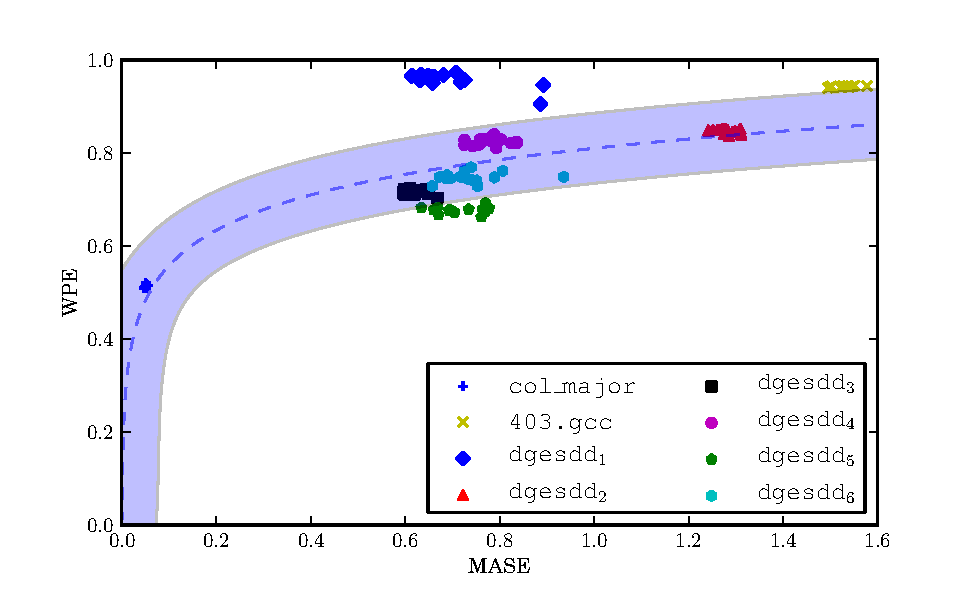
\includegraphics[width=\columnwidth]{figs/new_prediction_vs_entropy_autolog}
  \caption{Weighted permutation entropy vs. mean absolute scaled error
    (MASE) of the best prediction of each time series.
%
% (across all trials and all prediction methods)
%
The dashed curve is a least-squares log fit of all the points except
those from {\tt dgesdd$_1$}, which we have excluded for reasons
explained in the text.  [[Say what the colored region is and why we
    included it.]]}
  \label{fig:wpe_vs_mase_best}
\end{figure}
As the plot shows, the best-case prediction error for each trace from
these eight systems is roughly proportional to the log of the weighted
permutation entropy, which is consistent with our first conjecture.
The dashed line in the figure, a least-squares fit of $y = a \log(b x
+ c)$ to these errors\footnote{with the exception of {\tt dgesdd$_1$},
  for reasons described below} captures this relationship between WPE
and prediction error\footnote{The logarithmic fit is appropriate here
  because any signal with zero entropy should be perfectly
  predictable, and so should ideally have a MASE value of zero.}.
This is not a formal result.  The forecast methods and data sets used
here were chosen to span the space of standard prediction strategies
and the range of dynamical behaviors, but they do not cover those
spaces exhaustively.  Our goal here is an\emph{empirical} assessment
of the relationship between predictability and complexity, not formal
results about a ``best'' predictor for a given time series.  There may
be other methods that produce lower MASE values than those in
Figure~\ref{fig:wpe_vs_mase_best}, but the sparseness of the points
above and below the curve in this plot strongly suggests a pattern of
(inverse) correlation between the underlying predictability of a time
series and its WPE.  The rest of this section describes our results in
more detail---including the measures taken to assure meaningful
comparisons across methods, trials, and programs---and elaborates on
the meaning of the dashed curve in the figure.

Figure~\ref{fig:wpe_vs_mase_all} shows WPE vs. MASE plots for the full
set of experiments.
\begin{figure}
  \centering
%    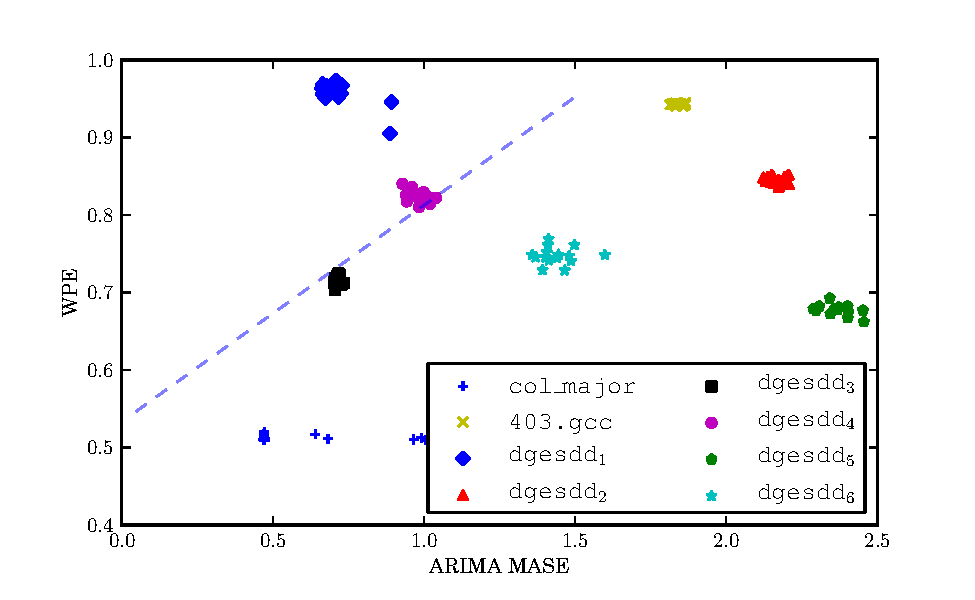
\includegraphics[width=\columnwidth]{figs/ARIMA_prediction_vs_entropy}
%    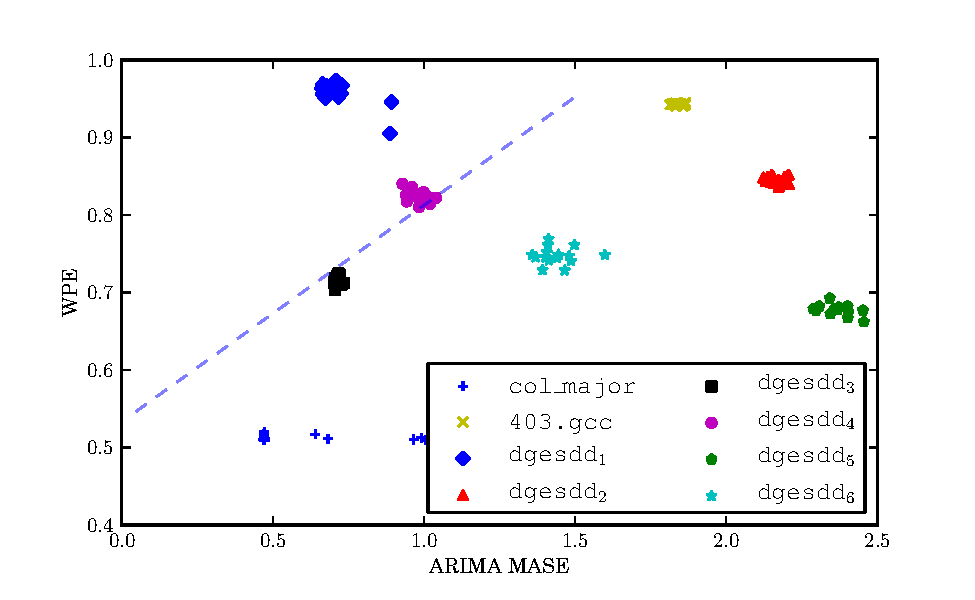
\includegraphics[width=\columnwidth]{figs/ARIMA_prediction_vs_entropy}
%    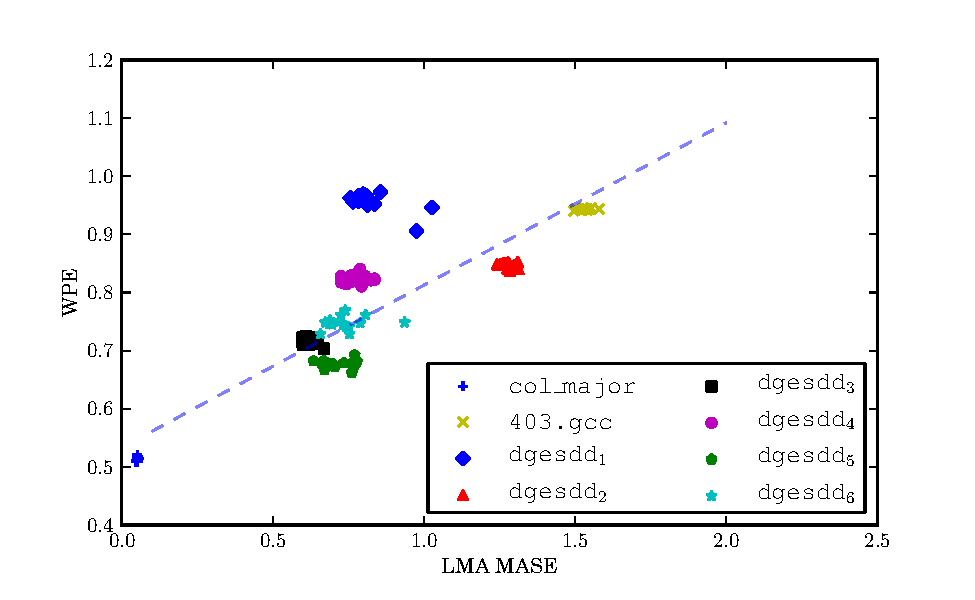
\includegraphics[width=\columnwidth]{figs/LMA_prediction_vs_entropy}
  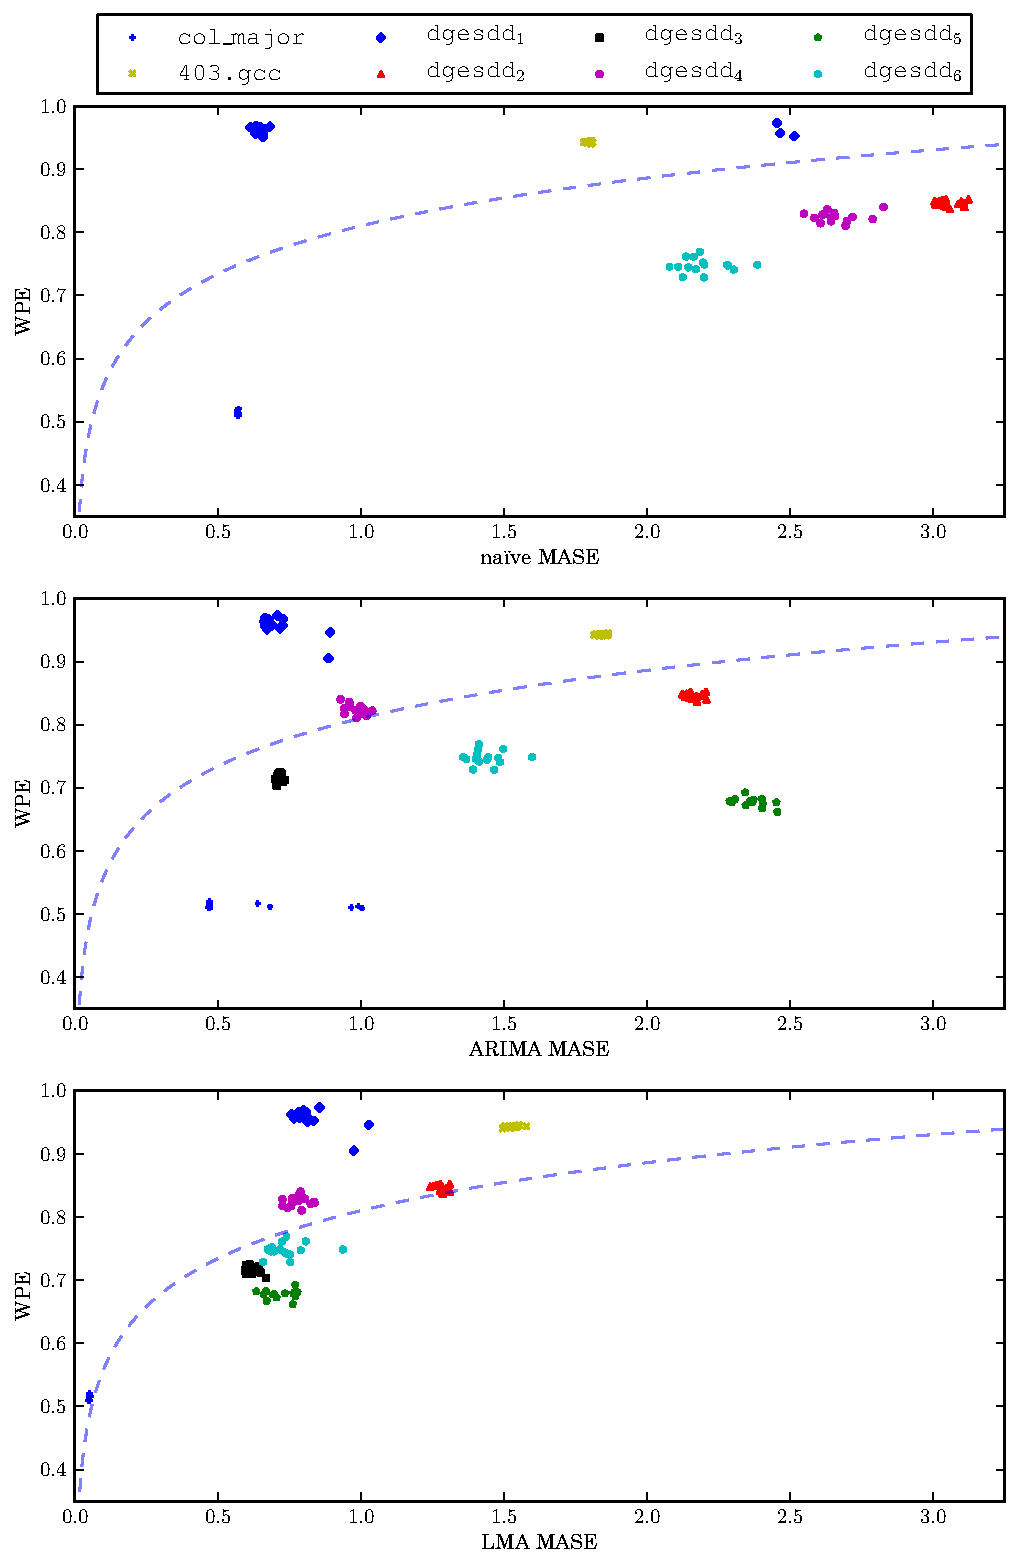
\includegraphics[width=\columnwidth]{figs/new_predictions_vs_entropy3}
\caption{WPE vs. MASE for all trials, methods, and systems---with the
  exception of \svdone, \svdthree, and \svdfive are omitted from the
  top plot for scale reasons.
%
% ; their MASE scores are $2.676 \pm 4.328$, $31.39 \pm 0.282$, and
%   $20.87 \pm 0.192$ respectively.
%
Numerical values, including means and standard deviations of the
errors, can be found in Table~\ref{tab:error}.  The dashed curve [[and
    shaded regions?  need to check this throughout the text and in all
    captions after we finalize the plot]] is the same as in the
previous figure.  }
    \label{fig:wpe_vs_mase_all}
\end{figure}
There are 15 points in each cluster, one for each trial.  (The points
in Figure~\ref{fig:wpe_vs_mase_best} are the leftmost of the points
for the corresponding trace in any of the three plots in
Figure~\ref{fig:wpe_vs_mase_all}.)  The WPE values do not vary very
much across trials.  For most traces, the variance in MASE scores is
low as well, resulting in small, tight clusters.  In some
cases---AutoARIMA predictions of {\tt col\_major}, for instance---the
MASE variance is larger, which spreads out the clusters horizontally.
The distribution of the cluster \emph{positions} is quite different in
the three plots.  The mean MASE scores of predictions generated with
the nonlinear LMA method are generally closer to the [[dashed curve]];
the AutoARIMA method clusters are more widely spread, the \naive ~clusters
even more so.  This geometric validation of the second conjecture in
this paper is discussed in more detail in the following paragraphs.

Though \col is a very simple program, its dynamics are actually quite
complicated, as discussed in Section~\ref{sec:intro}.  Recall from the
graphical representations in the left-hand column of
Figure~\ref{fig:forecast-example} that the \naive ~and AutoARIMA
prediction methods do not perform as well on this signal as the
nonlinear LMA method.  The MASE scores of the \naive ~and AutoARIMA
predictions are $0.571 \pm 0.002$ and $0.599 \pm 0.211$, respectively,
across all 15 trials.  That is, these methods are performing only
$\approx 1.7$ times better than the random-walk method, a primitive
strategy that simply uses the current value as the prediction.
However, the WPE value for the \col trials is $0.513 \pm 0.003$, which
is in the center of the complexity spectrum described in
Section~\ref{sec:intro}.

This disparity---WPE values that suggest a high rate of forward
information transfer in the signal, but predictions with comparatively
poor MASE scores---is obvious in the geometry of the top two images in
Figure~\ref{fig:wpe_vs_mase_all}, where the \col clusters are far to
the right of the [[dashed curve]].  \emph{This indicates that these
  methods are not leveraging the available information in the signal}.
The dynamics of \col may be complicated, but they are not
unstructured.  This signal is nonlinear and
deterministic\cite{mytkowicz09}, and if one uses a prediction
technique that is based a nonlinear model (LMA)---rather than a method
that simply predicts the running mean (\naive) or one that uses a
linear model (AutoARIMA)---the MASE score is much better: $0.050 \pm
0.001$.  This prediction is 20 times more accurate than a random-walk
forecast, which is more in line with the level of predictive structure
that the low WPE value suggests is present in the signal.

The [[dashed curve]] in Figures~\ref{fig:wpe_vs_mase_best}
and~\ref{fig:wpe_vs_mase_all} is a heuristic that captures the
argument at the end of the previous paragraph.  It can allow
practitioners to recognize when a prediction method is not well
matched to the task at hand: that is, when the time series has more
predictive structure than the method is able to use.  When the
predictions are well below [[that curve]] (as in the top and middle
images in Figure~\ref{fig:wpe_vs_mase_all}), one should try a
different method.  Conversely, the position of the LMA cluster---well
to the left of the other two, near the [[dashed curve]]---reflects
this method's ability to capture and exploit the structure that is
present in this signal.  [[Liz to wordsmith: Again, this curve was
    determined from a finite set of methods and data.  But we worked
    hard to make these experiments representative and comprehensive:
    forecast methods from simple to sophisticated; time-series data
    from a system whose behavior spans the dynamical behavior space.
    While we are cautiously opmistic about its generality, more
    exploration will be required to firm up that conclusion.  Say that
    Henon, Lorenz and SFI A fall within the colored region too, and
    that we're working on a broader study.]]

Note that the \col points (blue {\color{blue}$+$} icons) are clustered
very tightly in the lower left quadrant of the LMA and \naive ~MASE
vs. WPE plots, but spread out horizontally in the AutoARIMA plot.
This is because of the way that these models are built
\cite{autoARIMA}.  If a KPSS test of the time series in question
indicates that it is nonstationary, the AutoARIMA recipe adds an
integration term to the model.  This test gives mixed results in the
case of the \col process, flagging five of the 15 trials as stationary
and ten as nonstationary.  ARIMA models without an integration term
perform more poorly on this signal, which increases the error, thereby
spreading out the points\footnote{We tested this hypothesis by forcing
  the inclusion of an integration term in the five cases where a KPSS
  test indicated that such a term was not needed.  This action removed
  the spread, pushing all 15 of the \col AutoARIMA points in
  Figure~\ref{fig:wpe_vs_mase_all} into a tight cluster.}.
\alert{This paragraph probably needs more, in response to the ref's
  gritch about fitting.  We certainly want to call his attention to
  it, either way.}

The WPE of \svdfive ($0.677 \pm 0.006$) is higher than that of {\tt
  col\_major}.  This indicates that the rate of forward information
transfer of the underlying process is lower, but that time-series data
observed from this system still contain a significant amount of
structure that can, in theory, be used to predict the future course of
the time series.  As mentioned above, though, the effectiveness of any
prediction strategy depends on how well it leverages the information
that is available in the data: methods that use linear models, for
instance, may fail when applied to nonlinear processes.
%
% (This is the basis for the second conjecture above.)
%
This match between model and task is an issue in the \svdfive
experiments as well.  The MASE scores of the \naive ~and AutoARIMA
predictions for this system are $20.870 \pm 0.192$ and $2.370 \pm
0.051$, respectively: that is, 20.87 and 2.37 times worse than a
simple random walk forecast of the same signals\footnote{The \naive
  ~MASE score is large because of the bimodal nature of the
  distribution of the values of the signal, which makes guessing the
  mean a particularly bad strategy.  The same thing is true of the
  \svdthree signal.}.  As before, the positions of these points on a
WPE vs. MASE plot---significantly below and to the right of the shaded
region---should suggest to a practitioner that there is more structure
in this signal than the corresponding method is able to leverage, and
that a different method might do better.  Indeed, for \svdfive, the
LMA method produces a MASE score of $ 0.718\pm 0.048 $ and a cluster
of results that is much closer to the dashed curve on the WPE-MASE
plot.  Again, this validates our second conjecture: the LMA method can
capture and reproduce the way in which the \svdfive system processes
information, but the \naive ~and AutoARIMA prediction methods cannot.

The WPE of \gcc is higher still: $0.943 \pm 0.001$.  This system
transmits very little information forward in time and provides almost
no structure for prediction methods to work with.  Here, the \naive
~method performs best ($MASE=0.951 \pm 0.001$), simply because its
calculation of the mean filters out the noise in the signal.  Since
fitting a hyperplane using least squares should have similar effects,
the fact that LMA outperforms AutoARIMA ($1.530 \pm 0.021$ vs. $1.837
\pm 0.016$) is somewhat counterintuitive.  However, the small amount
of predictive structure that is present in this signal is nonlinear
(cf.,~\cite{mytkowicz09}), and LMA is designed to capture and exploit
that kind of structure.

\svdone---the dark blue segment of
Figure~\ref{fig:svd-ts-colored}---behaves very differently than the
other seven systems in this study.  Though its weighted permutation
entropy is very high ($0.957 \pm 0.016$), two of the three prediction
methods do quite well on this signal, yielding MASE scores of $0.827
\pm 0.076$ (LMA) and $0.714 \pm 0.075$ (AutoARIMA).  This pushes the
corresponding clusters of points in the bottom two images in
Figure~\ref{fig:wpe_vs_mase_all} well above the trend followed by the
other seven signals.  The MASE scores of the predictions that were
produced by the \naive ~method for this system, however, are highly
inconsistent.  The majority of the blue diamond-shaped points on the
top plot in Figure~\ref{fig:wpe_vs_mase_all} are clustered near a MASE
score of 0.6, which is better than LMA and AutoARIMA.  In five of the
15 \svdone trials, however, there were step changes in the signal.
The \naive ~method has a very difficult time with signals like this,
particularly if there are multiple step changes.  This raised the MASE
scores of these trials, pushing the corresponding points to the
right\footnote{This includes the cluster of three points near MASE
  $\approx 2.5$, as well as two points that are beyond the domain of
  the graph, at MASE 11.2 and 14.8.}, and in turn raising both the
mean and variance of this set of trials.

The effects described in the previous paragraph are also exacerbated
by the way MASE is calculated.  Recall that MASE scores are scaled
\emph{relative to a random-walk forecast}, which uses the current
value as the prediction.  This strategy works very badly on signals
with frequent, large, rapid transitions.  Consider a signal that
oscillates from one end of its range to the other at every step.  A
signal like this will have a low WPE, much like {\tt col\_major}.
However, a random-walk forecast of this signal will be 180 degrees out
of phase with the true continuation.  Since random-walk error appears
in the denominator of the MASE score, this effect can shift points
leftwards on a WPE vs. MASE plot, and that is exactly why the \svdone
clusters for AutoARIMA and LMA are above the dashed curve in
Figure~\ref{fig:wpe_vs_mase_all}.  This time series, which is shown in
closeup in Figure~\ref{fig:svdone-ts},
\begin{figure}[htbp]
  \centering
    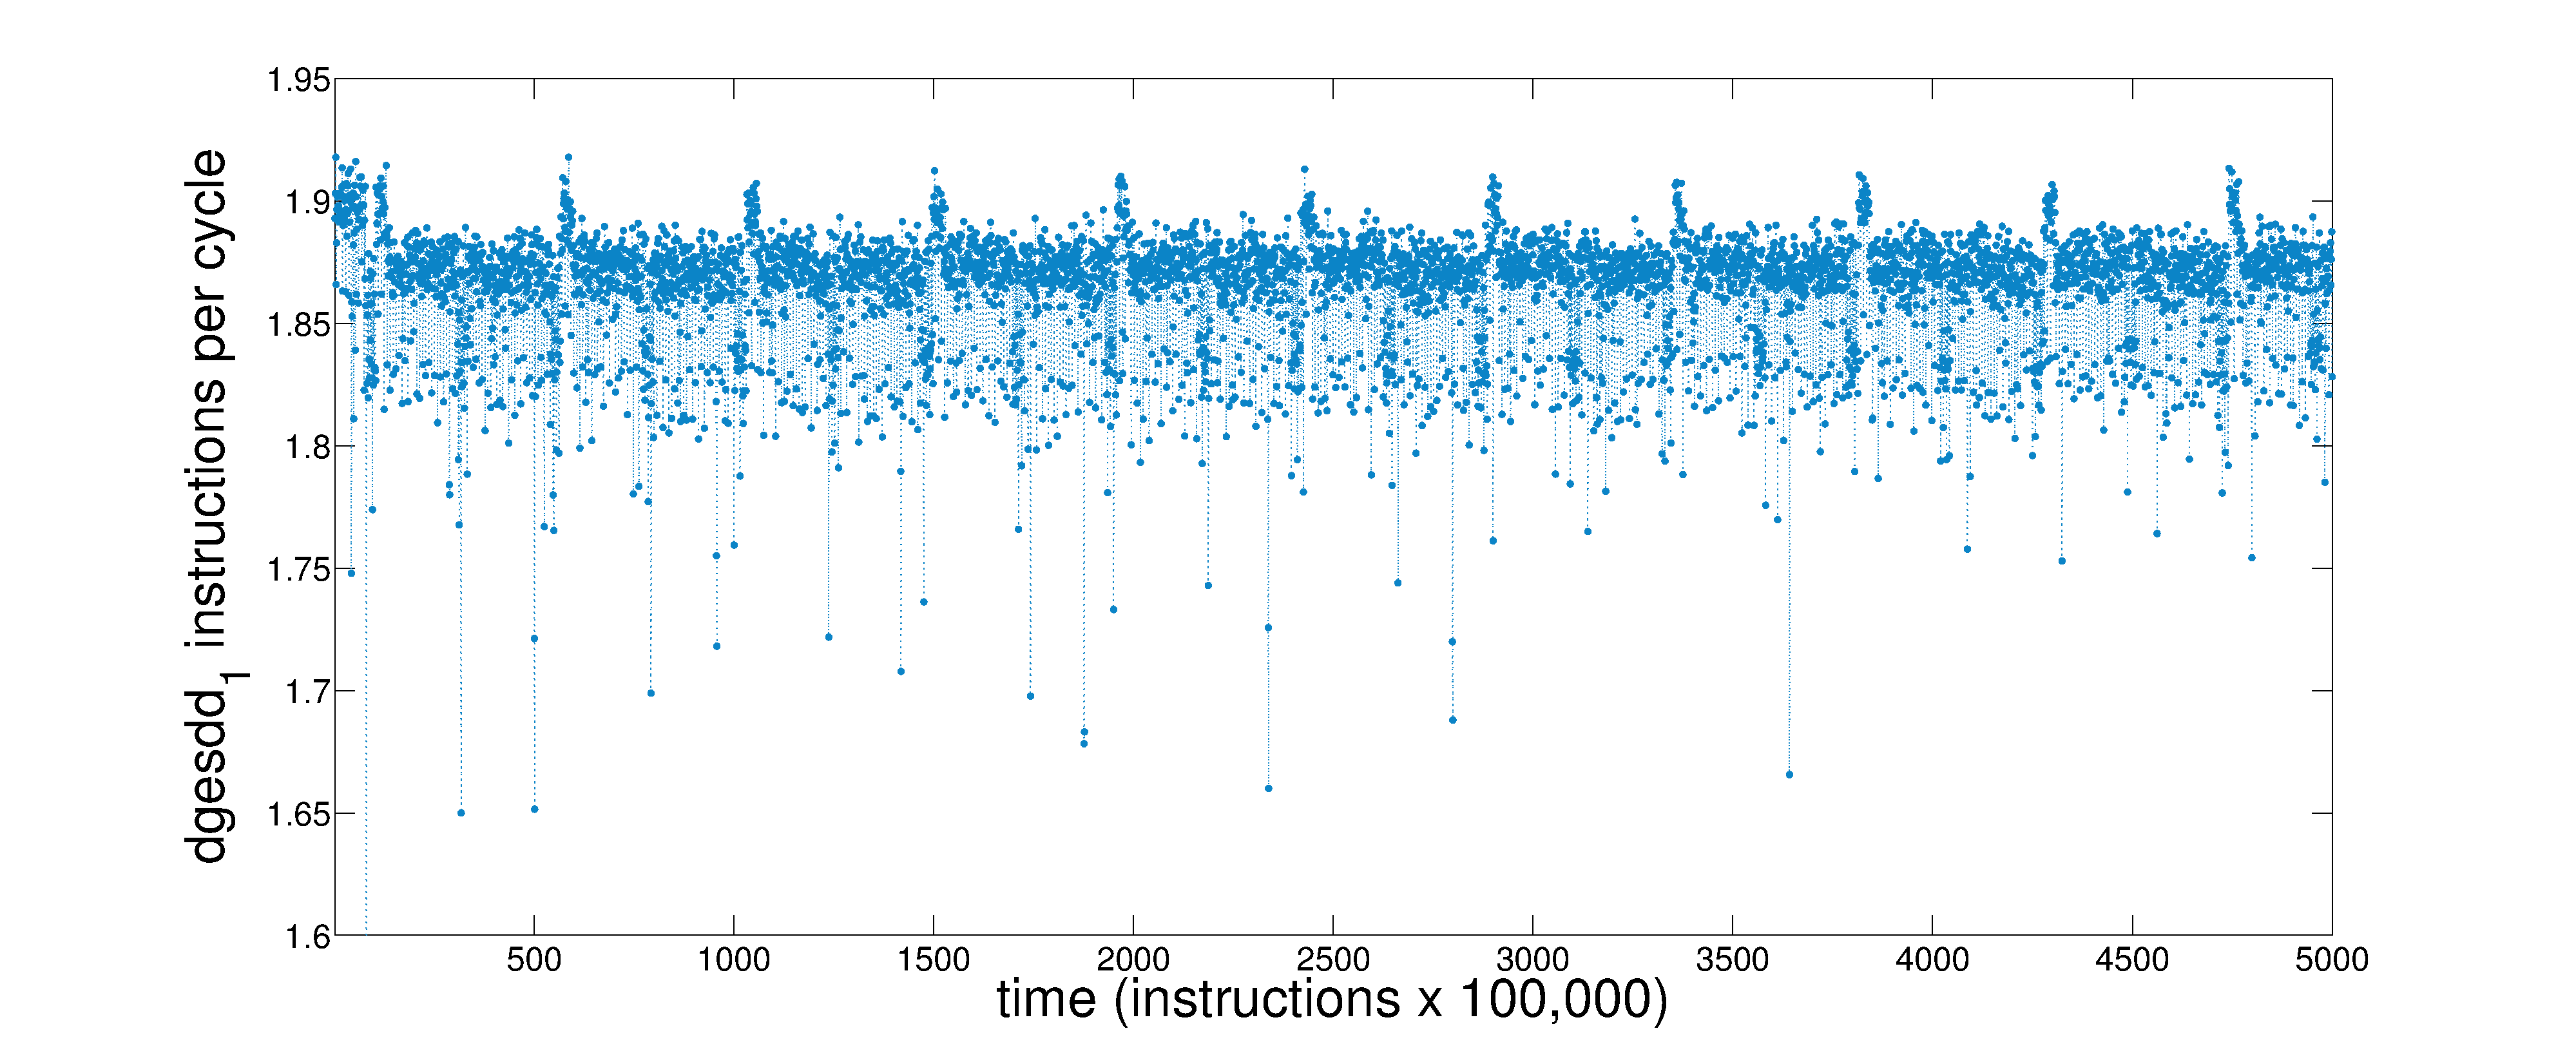
\includegraphics[width=\columnwidth]{figs/svdonets2}
\caption{A small portion of the \svdone time series}\label{fig:svdone-ts}
\end{figure}
is not quite to the level of the worst-case signal described above,
but it still poses a serious challenge to random-walk prediction.  It
is dominated by a noisy regime (between $\approx$1.86 and
$\approx$1.88 on the vertical scale in Figure~\ref{fig:svdone-ts}),
punctuated by short excursions above 1.9.  In the former regime, which
makes up more than 80\% of the signal, there are frequent dips to 1.82
and occasional larger dips below 1.8.  These single-point dips are the
bane of random-walk forecasting.  In this particular case, roughly
40\% of the forecasted points are off by the width of the associated
dip, which skews the associated MASE scores.  Signals like this are
also problematic for the \naive ~prediction strategy, since the
outliers have significant influence on the mean.  This compounds the
effect of the skew in the scaling factor and exacerbates the spread in
the \svdone MASE values.  For all of these reasons, we view \svdone as
an outlier and exclude it from the fit calculation of the dashed curve
in Figure~\ref{fig:wpe_vs_mase_best}.

[[Liz to wordsmith: Even though MASE has weaknesses, we concur with
    \cite{mase} that it is an effective way to compare prediction
    error across time series of different lengths and different
    scales.  Point to that paper for extensive evaluation and
    comparison wrt other metrics. We are in the process of repeating
    our own study with other metrics, other forecast methods, and
    time-series data from other systems.  Segue to next section.]]

%This portion should justify the following claim%%%%%%%%%%%%%%%%%%%%%%
%\item The way structure/information/complexity is processed internally by a given process plays a crucial role in predictability.
%%%%%%%%%%%%%%%%%%%%%%%%%

%In Figures~\ref{fig:lma_pred_vs_ent} and \ref{fig:arima_pred_vs_ent} we directly compare the performance of the LMA and ARIMA prediction methods (respectively) to the value of the weighted permutation entropy for all runs of each program under consideration. The LMA MASE values are largely similar to those of the best predictions, primarily because LMA often performed superior to ARIMA (and the na\"ive method). On the other hand, the ARIMA MASE values are largely uncorrelated with WPE values. As was hinted at while discussing the previous results, the fact that ARIMA is uncorrelated with WPE brings about an interesting perspective on information transfer and WPE. The WPE is sensitive to both linear and nonlinear structure. When you have a low WPE and a high ARIMA it could be that the structure WPE is picking up is simply nonlinear structure that LMA can handle but ARIMA cannot. So while ARIMA is consistently out performed by random walk,  there is plenty of structure present as suggested by WPE and taken advantage of by LMA but since it is nonlinear ARIMA can't take it into account and does bad.



%is in large part one of the major findings of this work. More specifically, say we tried to predict an arbitrary noisy real-valued time series with an ``out-of-the-box" prediction strategy like ARIMA as proposed in \cite{autoArima} and say we got inconsistent and bad forecasts, (i.e., perform worse than the na\"ive random walk strategy ($MAS>1$). How do we determine if the prediction strategy is not adequate for the prediction task, or if the signal is simply too complex to predict. If a signal is too complex and too little forward information transfer is present we may not be able to do better than the random walk, in which case we should not worry ourselves over finding a more complicated prediction strategy. However, if we measure the complexity to be low, $\textrm{WPE}<0.85$ (see Fig.~\ref{fig:pred_vs_wpe}) we can most likely do much better than the random walk and should search for more adequate prediction strategies.


